\documentclass[lettersize,journal]{IEEEtran}
\usepackage{amsmath,amsfonts}
\usepackage{algorithmic}
\usepackage{algorithm}
\usepackage{array}
\usepackage[caption=false,font=normalsize,labelfont=sf,textfont=sf]{subfig}
\usepackage{textcomp}
\usepackage{stfloats}
\usepackage{url}
\usepackage{verbatim}
\usepackage{graphicx}
\usepackage{cite}
\usepackage{xcolor}
\usepackage{parskip}
\usepackage{amsthm}
\usepackage{soul}
\hyphenation{op-tical net-works semi-conduc-tor IEEE-Xplore}
% updated with editorial comments 8/9/2021

\begin{document}

\title{An investigation into the effectiveness and impact of a Continuous Delivery pipeline upon university-level games development teams}

\author{Frost Donovan}

\maketitle

\begin{abstract}
    % What's the problem? What am I looking at? How does that help solve the problem? 
    % Opening, Challenge, Action, Resolution 

    Continuous Delivery (CD) is a technique designed to increase reliability and consistency with delivery of builds. This can then help to increase frequency of testing, the accountability of the development team, as well as the teams transpareny and \textit{"all being on the same page ness"}. This can increase team moral as well as stakeholder confidence, as both are able to regularly see the current state and rate of progress for the project. This encourages regular analysis of development pace and project scope, both internal and external. \\
    This stakeholder confidence and awareness of scope is a common problem within student development teams, so this investigation will answer to what extent the deployment of a CD pipeline will help to reduce these problems.
\end{abstract}

\section{Introduction}
    \subsection{What is Continuous Delivery?}
        CD is an expansion of Continuous Integration (CI), a pipeline for the continuous integration of code, being developed on separate branches, into the main branch. This code is merged into the main branch and then tested to ensure there are no merge conflicts or obvious errors thrown from the combined code. Assuming all of these tests pass, this merged code is pushed to the project repository. A key part of this pipeline is that the entire process is automated, ensuring minimal time is wasted waiting for tests to run or code to be uploaded. \cite{ContDelIntro,CICDCD} \\
        CD takes this one step further, in that after a project passes through the CI pipeline, the code is then compiled, packaged, and further tests that require the project to be compiled can be run. These tests should not be run before other tests that don't require compilation due to Fail Fast principles \cite{shore2004fail,bamboo}. Assuming there are no failures during compilation or testing, the built program can then be uploaded to somewhere where it can be easily accessed. Here, it is important to make a distinction between Continuous Delivery, where the build is available internally but not to users, and Continuous Deployment, where the build is pushed straight out to the current product users.
        core to agile methodology \cite{agilemanifesto}

    \subsection{Benefits \& Drawbacks of CD}
        The primary benefit of CD is reduced cycle time - a reduction in the time it takes for a change in the project to happen and then for the user to have that change applied to their version of the software. This principle is core to the agile methodology, being the very first principle in the agile manifesto \cite{agilemanifesto}. This faster cycle time means that feedback from active users can be obtained much quicker, both on the effectiveness of bug fixes and also on new features. Agile is designed to avoid the pitfalls of Waterfall \cite{royce1987managing}, one of which is the commitment of significant time and/ or resources into features that either are unattainable, or not actually wanted by the user. While other agile methods, such as Scrum or Extreme Programming \cite{cohen2004introduction,agilewithscrum}, can be an important part of the agile process, the effectiveness of a development team in delivering \textit{value} is always going to be dependant on the speed and reliability with which user feedback can be obtained. \\
        A benefit of this fast cycle time is not only are players able to see these changes faster, but stakeholders and publishers are able to see development progress, both regularly and on demand. This can be a significant step to building trust between a development studio and publisher, especially if the studio is new or doesn't have an existing relationship with the publisher \cite{gamedevhandbook}. 

        Part of the CD pipeline is testing, with a suite of unit tests being run on the code as part of the build process. As this build process is run consistently, rather than all at once leading up to a main release, this means bugs are found incrementally, stopping the accumulation of technical debt, reducing the cost to fix bugs, and reducing stress on programmers by preventing an overwhelming influx of bugs. While these unit tests will likely catch a lot of bugs, some bugs will only be caught during human playtesting. This decreased cycle time means that human playtesting can happen sooner \& more regularly, and fixes are delivered to testers \& players almost immediately, rather than having to wait for the next release window.
        
        Another strength of a Continuous Delivery pipeline is that it is fully automated. This allows less developer time to be spent setting up build or test environments and manually going through the build process, and more time on actually creating the product. This can be a \textit{significant} time save, with some large scale projects reportedly taking weeks to set up environments ready to produce a release build \cite{paddy, ContDelIntro}. This system also significantly reduces the chance that there are any errors caused by mistakes during the build process as this build-release pipeline will have had many iterations of the product pass through it, before a major release deadline. This increases the reliability and stability of new releases.
    
\section{Background \& Supporting Literature}
    With these benefits in mind it raises two questions; If a CD pipeline is this important and valuable, is it being taught to new developers in further education? If it is, is it actually as effective in practice with student teams as it is in theory?

    There is limited literature relating to Continuous Delivery being implemented in an academic context, and \textit{no} literature that I could find of this being implemented in a game development context. Even upon reviewing a literature review on rapid releases \cite{mantyla2015rapid} there were \textit{no} references to this within a games development context. This lack of literature provides a problem when attempting to find evidence on the performance of CD pipelines, however does highlight a \textit{need} for further literature and case studies on the subject. There is even a lack of literature relating to the effectiveness of CD pipelines within an industry setting. 
    
    Relating to the effect of CD pipeline deployment in an industry setting, a literature review by M{\"a}ntyl{\"a} et al. \cite{mantyla2015rapid} carried out an investigation into firefox's transition "from a TR [Traditional Release] model of one release a year to an RR [Rapid Release] model where new releases come every 6 weeks" \cite[pg 2]{mantyla2015rapid}. This paper concluded that, while there are are many benefits of rapid releases in literature, in this case study the transition from traditional release to a rapid release process "[has] not significantly impacted the product quality" \cite[pg 40]{mantyla2015rapid}. It is worth noting however, that this conclusion has been drawn from an interview with a single Mozilla Firefox QA engineer, as well as the test execution data from 06/2006 to 06/2012. While this data allows a quantitative analysis of the number of tests run or bugs found, it neglects the qualitative side of quality testing, the user's opinion of the software, usability, and perceived work being put into the software. As such, while this case study can give insight into the quantitative effects, it has insufficient evidence to state that the "quality" of the product has not changed \cite{kan2003metrics}.

    

    Given this lack, the papers being reviewed will be based around CD implementation in the academic setting of software development, a parallel field, but one which notably consists much more heavily of code, rather than the more even mix of skills and disciplines that is present within a game development context. As such, these papers all have a lack of analysis on how developers other than programmers respond to a CD pipeline, another case where there is a clear need for further study and literature.


    Has this been done before in academic setting\cite{CDCourse2014,CDMobileDev,IndustryAcademyDenmark}? 
    Links to other things - CI\cite{CICDCD}, Unit tests, regular product reviews, stakeholder (supervisor) confidence, git flow \cite{gitBranching}
    Best practices\cite{duvall2007continuous}? 

\section{Research Question}
    From the above sources, there is a clear need for research into the practical effects of a Continuous Delivery pipeline within game development and game development education. From this knowledge, I propose this initial investigation into the effects of a Continuous Delivery pipeline upon university-level games development teams, with a focus on the confidence of the team, as well as the confidence of the team's academic supervisor in their team. 
    This is purposefully broad, with the aim of encouraging and supporting further research into the topic. Given this, the following hypothesises will be investigated.

    \begin{enumerate}
        \item \label{h1} The use of a CD pipeline will increase a supervisors confidence in their team's ability to deliver a new, working build each week. (Q.S1)
        \item \label{h2} The team's confidence and the supervisors confidence in being able to achieve everything within the scope of the project will be much more closely related with the use of a CD pipeline.(Q.S2,St1 plotted against time)
        \item \label{h3} A CD pipeline will help developers understand the current state of the project (Q.St2)
        \item \label{h4} A CD pipeline will help developers to always know why the work they are doing is being done (Q.St3)
        \item \label{h5} A team using a CD pipeline will refine their scope more often (Q.St4)
        \item \label{h6} A team using a CD pipeline will do more playtesting
    \end{enumerate}

\section{Research Methodology}
    \subsection{Experimental Design}
        Environmental variation will be accounted for as all student team's within the study will be taken from the same population, Falmouth University Game's Academy. There may, however, be a relevant strata within this population that is not being accounted for, and that is the academic year the development team is in. This is discussed more in the fourth paragraph of the Limitation's section.
    
    \subsection{Limitations}
        The primary limitation in this study is a limited population size to draw from, which could be solved by increasing the duration of the study. If this study were to be expanded, I would ideally like to follow team's from their first year all the way through to graduation, introducing half of the teams to the CD pipeline immediately and then tracking their results, feedback, and attitudes across all three years against the control groups. This could also be done across multiple cohorts, providing increased statistical significance and helping to account for random variation between different team's cohesion and skill level. I would be cautious of instead increasing the population available to the study by reaching out to and running the study with multiple institutions. Due to the potentially significant environmental variation between institutions, both in staffing, course format, team agency, and an incredibly high number of other things, team's from different institutions would fall within different strata, meaning it could likely not reliably be treated as a single data set. \\
        If the study were to be run over an increased time span in this way, I can foresee a technical and potentially ethical concern that would require due consideration when designing the study.
        
        For the technical concern, game development team's within Falmouth University Game's Academy are not the same each year, they are quasi-randomised. This would mean it would be practically impossible to track the same 'team' across multiple years. Potentially individuals who have taken part in the study could be tracked, even if their team was not selected as an experimental group in the following year. Seeing if these individuals then implement their own CD pipelines could be a revealing statistic to look at as it would potentially give a measure of \textit{perceived} value, if not actual value. If this did occur then control groups would effectively be becoming experimental groups, potentially making a statistically sound comparison harder. \\
        The potential ethical problem could be if the initial results point towards a CD pipeline affecting a students \textit{grade}, how is that then handled. Does the experiment carry on as planned, potentially wilfully disadvantaging particular groups of students? While I am uncertain if this would be considered an ethical problem by an ethics board, it could likely provide a moral problem for those involved in running the study. A potential solution could be that those running the experiment would have to be kept in the dark about it's results while it was ongoing, in order to prevent any bias or conflict of interest. \\
        While these points would certainly require due consideration for a future study, they are not a concern for this initial study.

        A second limitation is that of resources available to those conducting the study. Ideally, every team with a CD pipeline deployed would have support to help customise the pipeline, supporting the team in building custom processes and writing robust unit tests to e executed within the pipeline. This would likely give the most 'accurate' imitation of a CD pipeline under industry conditions, however it is not possible to provide that level of support to all experimental team's. This is due to the research team being a singular individual whom has other commitments, and also lacks the experience to guide teams in writing unit tests effectively.

        A third limitation is the limited population size available to draw from, and the existence of four substrata within this population. Due to the reasons discussed in the first paragraph of this section, it is not possible to increase the available population size. The four substrata present are  the four academic years within Falmouth University Game's Academy. These are three undergraduate years, and a master's year. \\
        The environmental variation within these substrata will be minimised due to all students being of the same institution, but there will still be variation across several factors. The primary variation's will be in experience, which with minimal exceptions will increase as years progress, as well as team size, with masters team's being smaller than the average undergraduate team. \\
        A team's stage within the four stages of team development \cite{tuckman1965developmental} also has the potentially to vary significantly between a first year and a third year team. First year teams are quasi-randomised, with the intention of giving team's an even distribution of skills while putting students into a group with new people. This means the chance of a first year team having never worked together before is very high. Entering their second year student's are given more agency to choose who they work with in a development team, and then for third year student's are given complete agency to create team's with whomever they wish. This mean's that in second and especially third year team's are more likely to of worked with at least some members of the team before, allowing them to progress much quicker through Tuckman's model, or skip stages entirely to reach the most productive later stage's quicker.

    \subsection{Sampling}
        Mix of convenience \& voluntary response sampling of fal uni ga team's as all team's are eligible to take part. convenience sampling will be used by speaking to team's that are within the ga building, explaining study and asking them to take part. in theory this should give access to entire population, although given the current circumstances with Covid \cite{bbcomicron} some team's may have opted to work fully remotely, so would not be caught by this sampling method.\\
        As such, accompanying this method will be a batch of voluntary response sampling. Email shall be sent to all current student's within the ga, briefly detailing the study and asking students to take part. 

        sParticipant teams will then be evenly split between experimental groups who will be given the CD pipeline and control groups. which team's are control groups will be random. This random gathering of participants and assigning of control groups is purposefully to help account for random variation in steam skill and cohesion across all potential participant teams.
        
    \subsection{Data management plan}
        Data shall be collected using Microsoft Forms as it is GDPR compliant out the box. It will then be stored using Microsoft One Drive, another application that is GDPR compliant out the box.
        Data will be anonymised but matched after it has been collected, with participants names matching to unique ID numbers. The data will then be stored with this ID, rather than anything identifying like a name or email.
    
    \subsection{Data Analysis}
        All six hypothesis will be analysed using ANOVA with repeated measurements \& between factors. This is an expansion of the dependant t test \cite{carvadiaANOVA} which allows us to utilise the repeat measurements we will be taking. As we will be running this study with two distinct groupings of teams; teams that have access to the CD pipeline, and teams that do not (and thus are in the control group), this allows us to use the 'between factors', rather than 'within factors' test \cite{carvadiaANOVA}. \\
        Having determined an appropriate test type, we can then make use of GPower Software\cite{faul2007g,faul2009statistical}, alongside a comprehensive GPower guide \cite{gpowerguide}, to determine an effective sample size. First, we must provide the software with a number of parameters, which at this stage will be estimates based on our expected results, although after our data has been gathered we will revisit this and calculate these values in order to calculate the actual power of our results. The variables, along with the values we will be providing, are as follows.\\

        \subsubsection*{Effect Size f}
            This is the expected effect size we expect to see from our intervention. We are using a value of 0.4 here as this is the recommended value for a large effect size \cite{cohen1992power}, and as we are investigating practical relevance we care far more about large effects than effects that would be too small to provide practical relevance.\\

        \subsubsection*{$\alpha$ error probability}
            This will remain at the default value of 5\% as this is our probability of getting a type I error, also known as a false positive\cite{errortype}.\\

        \subsubsection*{Power}
            As this study is intended as an exploratory study, we will be accepting a power of 0.8. This will enable us to say with an 80\% certainty that we will not get a Type II error, also known as a false negative\cite{errortype}.\\

        \subsubsection*{Number of groups}
            We will have two groups, our control group who have no access to a CD pipeline, and our experimental group who are provided with the CD pipeline.\\

        \subsubsection*{Number of measurements}
            We are planning on collecting eight sets of measurements, one every two weeks from January through to March.\\
            
        \subsubsection*{Correlation among repeated measures}
            We will be using the default value of 0.5 here. This is the recommended value for a moderate to high correlation \cite{gpowerguide} which is to be expected. We will not be using a higher value as we expect some level of variation due to the project moving through a significant part of its lifecycle during the period we are monitoring, as well as variation due to team's becoming more accustomed to working together and moving through the four stages of team forming \cite{tuckman1965developmental}. This will be especially prevalent in first and second year teams, as they are more likely to of not worked together due to how Falmouth University Game's Academy operates.

        Using these values, we receive a required sample size of thirty participants (see figure \ref{ANOVArepeatedbetween}). While this is realistic for hypothesis regarding individuals, see hypothesis \ref{h3} and \ref{h4}, this will be more challenging for the rest of the hypothesises as they relate to teams as a whole, meaning we would require 30 \textit{teams}, not individuals. This is potentially possible, but will require the participation of two thirds of the entire population of Falmouth University Game's Academy.

        \begin{figure}[h!]
            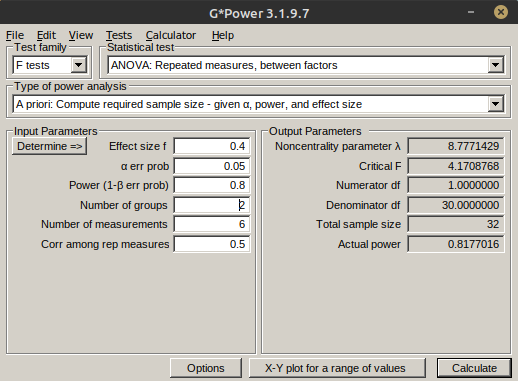
\includegraphics[width=\columnwidth]{Images/ANOVA_2.png}
            \caption{Screen capture from GPower software showing sample size calculation for an \textit{ANOVA: repeated measurements, between factors} test}
            \label{ANOVArepeatedbetween}
        \end{figure}

    \subsection{Ethical Considerations}
        Due to the nature of this research, there are minimal ethical considerations that need to be taken into account. The participants will not be exposed to any potential risks outside of what they would experience under normal circumstances, although an effort has been made to keep the feedback form fairly condensed. This is to minimise any increased stress that the commitment of having to fill out the form may cause.
    
    \section{Appendix}
    Data analysis code, supporting screenshots, list of unit tests \& testing plan

\section{Artifact}
    briefly describe artifact
    make a brief note on quality assurance
    link to git repo
    show off any screenshots or code excerpts

    More interested in what and how at this stage

    two repo link - one with artifact to easily show off then give link to show it embedded in main project
    \subsection{What will be made}
        CD pipeline utilising Github Actions. Tool to set up secrets? Would be sick \url{https://docs.github.com/en/rest/reference/actions#secrets} \\
        Continuous delivery or continuous deployment? Scope as deployment would need to include itch integration w/ butler, although it looks relatively simple to set up.
        Auto-upload to steam \& itch! \url{https://itch.io/docs/butler/}

    \subsection{How will I ensure Quality}
        Quality control. Roadmap? Unit Testing? Integration testing?

    \subsection{How will I create it}

    \subsection{Why will this answer the questions}

\bibliographystyle{ieeetr}
\bibliography{bibliography}

\end{document}